\documentclass[journal]{IEEEtran}

\usepackage{amsmath,amssymb}
\usepackage{graphicx}
\usepackage{booktabs}
\usepackage{hyperref}
\usepackage[utf8]{inputenc}

\graphicspath{{figures/}}

\begin{document}

\title{Predictive Amortized KV-Caching for Low-Latency Edge LLMs in Augmentative and Alternative Communication}

\author{
\centering
Arjit Tripathi\\
\textit{arjit.tripathi2023@vitstudent.ac.in}

\vspace{1em}

\begin{minipage}[t]{0.45\textwidth}
\centering
Medha Sriram\\
\textit{medha.sriram2023@vitstudent.ac.in}
\end{minipage}
\hfill
\begin{minipage}[t]{0.45\textwidth}
\centering
Heer Shah\\
\textit{heer.shah2023@vitstudent.ac.in}
\end{minipage}
}

\maketitle

% ===========================================================================
% ABSTRACT
% ===========================================================================
\begin{abstract}
Augmentative and alternative communication (AAC) devices that leverage large language models can generate context-aware responses tailored to a user's environment, but the computational cost of processing contextual prompts at inference time introduces latency that is incompatible with real-time communication. We present Context-Aware Predictive KV-Cache Priming (CAP-KVC), a system that amortizes this cost by using environmental sensor signals---GPS, Bluetooth Low Energy proximity, and time of day---to predict the user's likely context and pre-compute the corresponding key-value cache tensors during idle periods. At inference time, the pre-computed cache is restored from persistent storage in 2.63~ms on average, and only the user's intent tokens are processed by the language model. Evaluated on a OnePlus~11R with Qwen2.5-0.5B-Instruct (Q4\_K\_M), CAP-KVC reduces end-to-end inference latency by 1.32$\times$ at comparable context length and by 4.59$\times$ as context grows to approximately 500~tokens, relative to standard retrieval-augmented generation. The system is implemented as a complete Android application with a C++/JNI inference backend, a bounded KV cache residency manager supporting three simultaneous states within a 118.7~MB native heap budget, and a multimodal intent classification pipeline combining surface electromyography and gaze tracking through late fusion. We report all measurements, acknowledge limitations including single-device evaluation and synthetic fusion training data, and release the complete implementation for reproducibility.
\end{abstract}

\begin{IEEEkeywords}
Augmentative and alternative communication, key-value cache, large language model, edge inference, predictive caching, electromyography, gaze tracking, sensor fusion.
\end{IEEEkeywords}

% ===========================================================================
% I. INTRODUCTION
% ===========================================================================
\section{Introduction}
\label{sec:introduction}

Augmentative and alternative communication (AAC) devices are essential for individuals with severe motor impairments who have lost the ability to produce natural speech. For people with conditions such as amyotrophic lateral sclerosis (ALS), these devices often represent the primary means of expressing basic needs, participating in conversation, and maintaining social agency. The responsiveness of an AAC system directly affects the user's ability to communicate in real time: delays of even a few seconds can disrupt conversational turn-taking and erode the communicative experience~\cite{beukelman2020}.

Recent advances in model quantization and optimized inference runtimes have made it feasible to run small language models on mobile hardware, opening the possibility of generative AAC responses that go beyond pre-defined phrase boards. A context-aware language model can generate responses tailored to the user's current environment---for example, producing medical terminology when in a hospital ward, or casual greetings when a caregiver arrives. However, this contextual awareness comes at a cost: the system prompt encoding the environmental context must be processed by the model before any response can be generated. For a prompt of $N$ tokens, this prefill phase adds $O(N)$ latency at inference time, creating a direct tension between response quality and user-perceived responsiveness.

In server-side deployments, KV cache reuse techniques such as prefix sharing and paged attention amortize prefill costs across concurrent requests from multiple users. These techniques are not directly applicable to edge AAC devices, which serve a single user on a single device with no shared request stream. In many such deployments, the contextual prompt is reprocessed during each inference request.

This paper presents \textbf{Context-Aware Predictive KV-Cache Priming (CAP-KVC)}, a system that resolves this tension by decoupling the context prefill from the inference request path. CAP-KVC uses environmental sensor signals---GPS location, Bluetooth Low Energy (BLE) proximity beacons, and time of day---to predict which semantic context the user is most likely to need. It then executes the prefill during idle periods, serializes the resulting KV cache tensors to persistent storage, and restores them at inference time. The user-facing inference path processes only the short intent tokens, reducing the inference-time prefill to a cache restoration operation that completes in under 3~ms.

The system is implemented as a complete Android application with a C++/JNI inference backend based on \texttt{llama.cpp}, a Kotlin orchestration layer managing cache residency and sensor-driven routing, and a multimodal intent classification pipeline combining surface EMG and gaze tracking inputs through a late fusion architecture.

The contributions of this paper are as follows:

\begin{enumerate}
    \item \textbf{CAP-KVC Architecture:} A predictive KV cache priming system that amortizes context prefill costs by leveraging environmental sensors for background cache state selection and persistence. We observe a 1.32$\times$ to 4.59$\times$ reduction in end-to-end inference latency compared to standard RAG-inline inference on a mobile device, with cache restoration completing in 2.63~ms on average.

    \item \textbf{Edge-Native Implementation:} A complete, deployable Android implementation comprising a scalar-only JNI boundary (8~native functions), a reentrant-lock concurrency model for safe native state access, an LRU cache residency manager bounded to 3~simultaneous KV states, and a deterministic context routing engine using a convex sensor scoring function.

    \item \textbf{Sensor-Driven Context Routing:} A closed-form scoring function that dynamically combines temporal, spatial, and BLE proximity signals with reliability-adaptive weighting, including hysteresis-gated drift detection to prevent cache thrashing under noisy sensor conditions.

    \item \textbf{Multimodal AAC Pipeline:} A fusion architecture combining CNN-LSTM sEMG embeddings with MediaPipe gaze tracking through late fusion, deployed on-device via ONNX Runtime, with a controlled ablation study comparing late fusion against cross-attention.
\end{enumerate}

\subsection{Research Questions}
\label{sec:rqs}

This work addresses the following research questions:

\begin{itemize}
    \item \textbf{RQ1} (Latency Amortization): To what extent does CAP-KVC reduce end-to-end inference latency relative to conventional RAG-inline inference on mobile hardware?
    \item \textbf{RQ2} (Memory Viability): What memory overhead is required to maintain bounded multi-state KV cache residency on an edge device?
    \item \textbf{RQ3} (Multimodal Intent Classification): Does late fusion provide superior multimodal intent-classification performance compared to cross-attention under the evaluated conditions?
\end{itemize}

The remainder of this paper is organized as follows. Section~\ref{sec:related} surveys related work in KV cache optimization, edge LLM deployment, and assistive technology. Section~\ref{sec:methodology} describes the CAP-KVC methodology. Section~\ref{sec:implementation} details the Android implementation. Section~\ref{sec:experiments} presents the experimental setup. Section~\ref{sec:results} reports and discusses the results. Section~\ref{sec:conclusion} concludes with a summary of findings and limitations.

% ===========================================================================
% II. RELATED WORK
% ===========================================================================
\section{Related Work}
\label{sec:related}

\subsection{Augmentative and Alternative Communication}
\label{sec:related_aac}

AAC devices serve individuals with severe motor impairments, including those caused by amyotrophic lateral sclerosis (ALS), cerebral palsy, and acquired brain injuries. Traditional AAC systems rely on grid-based symbol selection interfaces that require deliberate motor actions such as switch scanning or eye-gaze pointing~\cite{beukelman2020}. While effective, these interfaces constrain communication to pre-defined vocabularies and impose high cognitive load during message construction.

Recent work has explored integrating language models into AAC workflows to provide generative communication support. Approaches include word and phrase prediction~\cite{vertanen2015}, context-sensitive sentence completion, and full open-vocabulary generation. However, deploying language models on edge devices introduces a fundamental tension between response quality (which improves with model size and context length) and latency (which degrades with both).

\subsection{Edge Deployment of Large Language Models}
\label{sec:related_edge}

The deployment of transformer-based language models on mobile and embedded hardware has been enabled by advances in model quantization and optimized inference runtimes. Post-training quantization to 4-bit precision~\cite{dettmers2022,frantar2022} reduces both memory footprint and arithmetic intensity, enabling sub-billion parameter models to run on smartphone SoCs. Inference frameworks such as \texttt{llama.cpp}~\cite{llamacpp} and MLC-LLM~\cite{mlcllm} provide ARM NEON--optimized kernels and memory-mapped model loading for efficient mobile execution.

Despite these advances, the prefill phase of autoregressive inference remains a latency bottleneck. For a prompt of $N$ tokens, the prefill requires $O(N)$ forward passes through the model before the first output token can be generated. In AAC contexts, where system prompts encoding environmental and medical information may span hundreds of tokens, this prefill cost can dominate the user-perceived response time.

\subsection{KV Cache Optimization}
\label{sec:related_kvcache}

The key-value (KV) cache stores the attention key and value tensors computed during the prefill phase, allowing subsequent tokens to attend to the full context without recomputation. Several lines of research have sought to reduce the memory and computational costs of KV cache management.

\textbf{Cache compression} methods reduce KV cache memory through selective eviction of less-important entries. Scissorhands~\cite{scissorhands} identifies and removes KV pairs corresponding to tokens with low cumulative attention scores. H$_2$O~\cite{h2o} extends this with a ``heavy hitter'' policy that retains high-attention tokens. StreamingLLM~\cite{streamingllm} maintains only a fixed-size attention window plus initial ``attention sink'' tokens to enable infinite-length generation. These methods operate at the token level within a single sequence and are complementary to the state-level caching proposed in this work.

\textbf{Prompt caching} systems amortize prefill costs by reusing cached computations across requests sharing common prompt prefixes. SGLang's RadixAttention~\cite{sglang} organizes cached prefixes in a radix tree for server-side multi-tenant reuse. vLLM~\cite{vllm} uses paged attention to share KV blocks across concurrent requests with common prefixes. These systems target cloud inference serving with multiple concurrent users and do not address the single-user, single-device edge deployment scenario.

\textbf{State management} approaches extend KV caching beyond single sessions. InfiniGen~\cite{infinigen} speculatively prefetches KV cache entries for predicted future tokens. CacheGen~\cite{cachegen} compresses and stores KV caches for reuse across sessions. The present work is most closely aligned with this family of approaches, differing in its focus on predictive state selection driven by environmental sensor signals rather than textual context alone.

\subsection{Multimodal Sensor Fusion for Assistive Technology}
\label{sec:related_fusion}

Combining EMG and gaze signals for human-computer interaction has been explored in several assistive technology contexts. EMG-based gesture classification using convolutional and recurrent architectures has been evaluated on public datasets including NinaPro~\cite{ninapro} and the Myo Armband dataset. Gaze-based interaction using facial landmark models such as MediaPipe~\cite{mediapipe} provides a complementary channel that does not require residual motor function. Late fusion and cross-attention architectures have been compared for combining heterogeneous sensor modalities in gesture recognition~\cite{ngiam2011}, with late fusion often preferred for its simplicity and robustness when modality reliability varies.

\subsection{Positioning of This Work}
\label{sec:positioning}

The present work differs from prior KV cache optimization research in two respects. First, it targets a single-user, single-device edge deployment where background computation during idle periods can be exploited for prefill amortization---an operational model that is unavailable in cloud serving scenarios. Second, it introduces environmental sensor signals (GPS, BLE, time) as the basis for predictive cache state selection, replacing the purely textual prefix-matching strategies used in cloud KV cache systems.

% ===========================================================================
% III. METHODOLOGY
% ===========================================================================
\section{Methodology}
\label{sec:methodology}

This section describes the design of the Context-Aware Predictive KV-Cache Priming (CAP-KVC) system and its integration within the AACBridge communication pipeline. The primary goal is to amortize the computational cost of contextual prompt ingestion on resource-constrained mobile hardware by executing it as a background process, prior to user interaction. Fig.~\ref{fig:architecture} presents an overview of the system architecture.

\begin{figure*}[t]
\centering
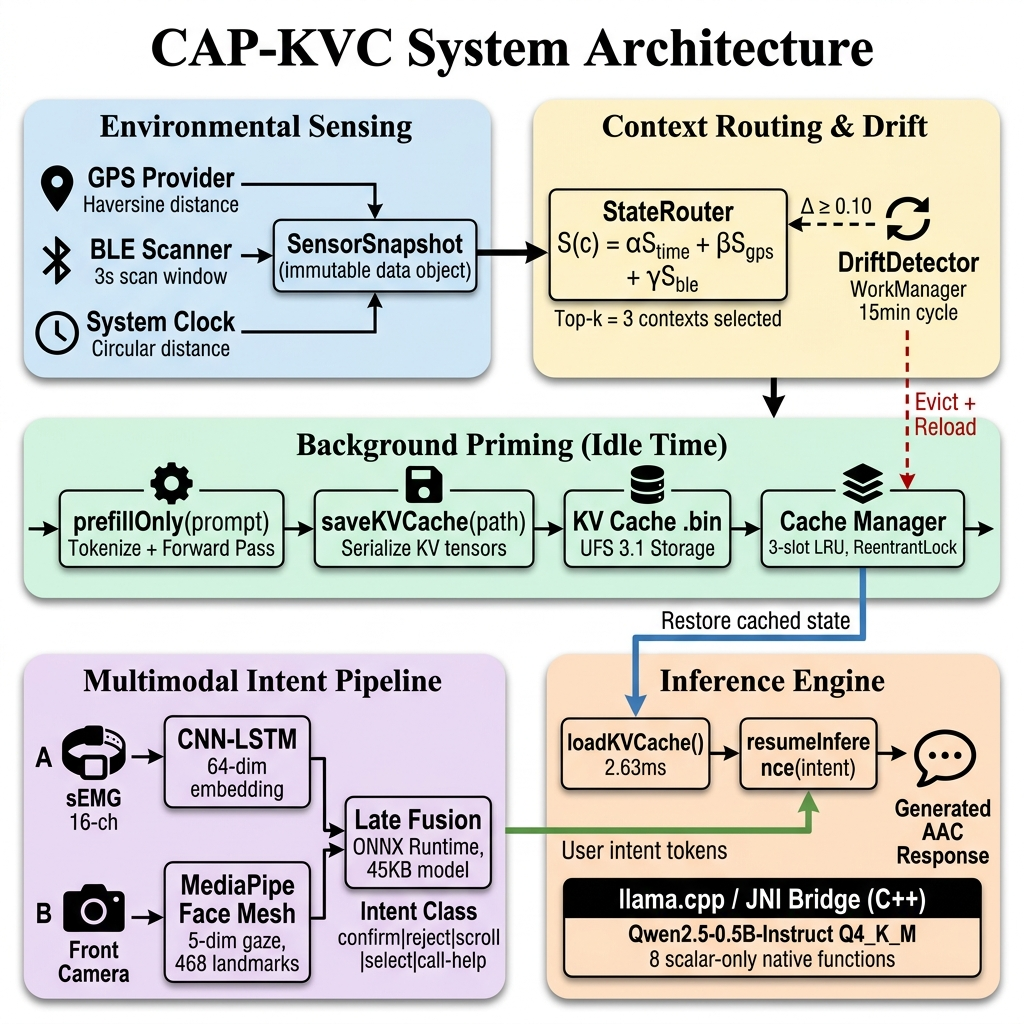
\includegraphics[width=0.85\textwidth]{figures/system_architecture.png}
\caption{CAP-KVC system architecture. Environmental sensors (blue) feed a deterministic scoring function that selects contexts for background priming (green). The multimodal intent pipeline (purple) combines sEMG and gaze inputs via late fusion. At inference time (orange), the pre-computed KV cache is restored and only intent tokens are processed by the llama.cpp/JNI backend. A periodic drift detector re-evaluates context relevance with hysteresis gating ($\Delta \geq 0.10$).}
\label{fig:architecture}
\end{figure*}

\subsection{Problem Formulation}
\label{sec:problem}

Consider a user $u$ operating an AAC device in a physical environment characterized by temporal, spatial, and proximity signals. Let $C = \{c_1, c_2, \ldots, c_M\}$ denote a finite set of pre-configured semantic contexts, each associated with a textual system prompt $p_i$ of length $N_i$ tokens. In conventional retrieval-augmented generation (RAG) pipelines, the system prompt $p_i$ is concatenated with the user's intent tokens and submitted to the language model at inference time, incurring an $O(N_i)$ prefill cost that directly adds to user-perceived latency.

CAP-KVC reformulates this as a scheduling problem: given a prediction of the user's most likely context $\hat{c}$ based on environmental signals, execute the prefill of $p_{\hat{c}}$ during idle periods and persist the resulting key-value (KV) cache tensors to persistent storage. At inference time, the system restores the pre-computed KV cache and appends only the user's intent tokens, reducing the inference-time cost from context-length-dependent prompt processing to a lightweight cache restoration operation whose cost is independent of the original prompt length $N_i$.

\subsection{System Execution Lifecycle}
\label{sec:lifecycle}

The system operates through a five-stage pipeline, where the first three stages execute asynchronously during background idle periods and the final two stages execute at user-interaction time:

\begin{enumerate}
    \item \textbf{Sensor Acquisition.} The system concurrently polls available hardware sensors---GPS, Bluetooth Low Energy (BLE), and the system clock---to construct an immutable \texttt{SensorSnapshot} representing the user's current environmental state.

    \item \textbf{Deterministic Context Routing.} The snapshot is evaluated by a \texttt{StateRouter} against all registered semantic contexts using a convex scoring function (Section~\ref{sec:scoring}). The top-$k$ highest-scoring contexts are selected for cache residency, where $k$ is bounded by a device-specific RAM constraint (Section~\ref{sec:residency}).

    \item \textbf{Background Cache Priming.} For each selected context not already resident in memory, the system executes a background prefill of its system prompt through the language model, serializes the resulting KV cache tensors to persistent storage, and registers the context as resident.

    \item \textbf{Resident Inference.} Upon user interaction, the pre-computed KV cache for the predicted context is restored from storage into native memory. The user's intent tokens are then appended and decoded, bypassing the context prefill entirely.

    \item \textbf{Drift Correction.} An asynchronous background daemon periodically re-evaluates environmental scores to detect changes in the user's physical context and triggers cache replacement when a new context scores sufficiently higher than the weakest resident context (Section~\ref{sec:drift}).
\end{enumerate}

\subsection{Multimodal Intent Classification}
\label{sec:fusion}

User intent is derived from two complementary input modalities, fused to produce a single classification decision that is then formatted as a textual prompt for the language model.

\subsubsection{Surface Electromyography (sEMG)}
A facial sEMG wearable provides 16-channel signals sampled continuously. Raw signals are segmented into fixed-length windows and processed by a CNN-LSTM classifier that extracts a 64-dimensional embedding vector. The CNN block applies three sequential Conv1d--BatchNorm--ReLU--MaxPool layers for temporal feature extraction, followed by a two-layer LSTM for temporal context modeling. The final hidden state is projected to a 64-dimensional space and L2-normalized to produce the EMG embedding.

\subsubsection{Gaze Tracking}
A front-facing camera feeds a MediaPipe Face Mesh model~\cite{mediapipe} that extracts 468 facial landmarks at frame rate. From these, the system computes a 5-dimensional gaze feature vector from the displacement between the nose tip (landmark 4) and the eye center (midpoint of landmarks 33 and 362):

\begin{equation}
\mathbf{g} = [d_x,\; d_y,\; |d_x|,\; |d_y|,\; \sqrt{d_x^2 + d_y^2}]
\label{eq:gaze_vector}
\end{equation}

\noindent where $d_x$ and $d_y$ are the horizontal and vertical displacements in normalized image coordinates. This vector captures both directional and magnitude information while remaining invariant to face scale. A dwell-based finite state machine maps sustained gaze fixation (exceeding 400ms on a target region) to one of five discrete AAC intent classes: \emph{confirm}, \emph{reject}, \emph{scroll}, \emph{select}, and \emph{call-help}.

\subsubsection{Late Fusion Architecture}
The EMG embedding $\mathbf{e} \in \mathbb{R}^{64}$ and the gaze vector $\mathbf{g} \in \mathbb{R}^{5}$ are fused through a late fusion architecture. The gaze vector is first projected to a 64-dimensional space via a two-layer MLP, then concatenated with the EMG embedding to produce a 128-dimensional joint representation. A final two-layer classifier maps this to 5-class intent logits:

\begin{equation}
\hat{y} = \text{MLP}_{64 \rightarrow 5}\big(\text{ReLU}\big(\text{MLP}_{128 \rightarrow 64}([\mathbf{e};\; \text{proj}(\mathbf{g})])\big)\big)
\label{eq:late_fusion}
\end{equation}

Late fusion was selected over a cross-attention alternative based on a pre-specified decision criterion: cross-attention must exceed late fusion F1 by more than 3\% (absolute) to justify its additional computational and parameter overhead. The ablation results (Section~\ref{sec:results_fusion}) did not meet this threshold.

\subsection{Deterministic Context Scoring}
\label{sec:scoring}

We employ a deterministic, closed-form scoring function rather than a learned predictor to ensure bounded CPU and battery consumption during background polling. A semantic context $c_i$ is scored against the current sensor snapshot as a convex combination of three environmental similarity scores:

\begin{equation}
S(c_i) = \alpha \cdot S_{\text{time}} + \beta \cdot S_{\text{gps}} + \gamma \cdot S_{\text{ble}}
\label{eq:scoring}
\end{equation}

\noindent where $\alpha + \beta + \gamma = 1$ and each weight reflects the estimated reliability of its corresponding sensor.

\subsubsection{Temporal Scoring}
The temporal similarity $S_{\text{time}}$ applies a Gaussian kernel to the circular distance between the current time and the context's expected activation time:

\begin{equation}
S_{\text{time}} = \exp\!\left(-\frac{d_{\text{circ}}(t, t_i)^2}{2\sigma^2}\right)
\label{eq:time_score}
\end{equation}

\noindent where $d_{\text{circ}}$ handles the 24-hour wraparound and $\sigma = 2.0$ hours accommodates typical schedule variability.

\subsubsection{Spatial Scoring}
The spatial similarity $S_{\text{gps}}$ applies an exponential decay to the Haversine great-circle distance between the current GPS coordinates and the context's anchor location:

\begin{equation}
S_{\text{gps}} = \exp(-\lambda \cdot d_{\text{haversine}})
\label{eq:gps_score}
\end{equation}

\noindent with $\lambda = 0.1$~m$^{-1}$, establishing a contextual boundary of approximately 100~meters.

\subsubsection{BLE Proximity Scoring}
The BLE similarity $S_{\text{ble}}$ evaluates the overlap between currently detected Bluetooth devices and a context's registered device topology, with RSSI values mapped through a sigmoid function.

\subsubsection{Dynamic Reliability Normalization}
The weights $\alpha$, $\beta$, and $\gamma$ are computed dynamically from raw sensor reliability estimates. Time maintains a fixed baseline weight ($w_t = 0.4$), guaranteeing that the normalization denominator $w_t + w_g + w_b$ is always positive. If GPS is unavailable ($w_g = 0$) or no BLE devices are detected ($w_b = 0$), the corresponding weight contribution is redistributed proportionally, preserving the convex property. Contexts scoring below a dead-state threshold of 0.01 are excluded from routing consideration.

\subsection{KV Cache Residency Management}
\label{sec:residency}

The system maintains at most $k$ KV cache states simultaneously resident in native memory, where $k$ is configured based on the target device's available RAM budget ($k = 3$ in the current deployment). KV cache states are mapped to native sequence slots managed by the underlying inference engine.

When a new context requires loading and all slots are occupied, the least-recently-used (LRU) state is evicted. Eviction is protected by a reference-counting mechanism: a state undergoing active inference holds a reference that blocks eviction until inference completes. The eviction loop waits for the reference count to drain to zero before releasing the native slot.

\subsection{Asynchronous Drift Detection}
\label{sec:drift}

Environmental sensors predict physical location but cannot detect whether the conversation topic has diverged from the cached context. A periodic background daemon (executing every 15 minutes via the Android WorkManager API) re-evaluates context scores using a lightweight sensor snapshot and compares them against currently resident states.

To prevent cache thrashing under noisy sensor conditions, state replacements are gated by a hysteresis margin: a candidate context must exceed the weakest resident state's score by at least $\Delta = 0.10$ before a cache swap is authorized. This prevents oscillatory eviction-reload cycles that would impose unnecessary I/O and prefill costs.

A separate offline ablation study evaluated the sensitivity of conversation-level drift detection to the sliding window size $k$ used for centroid computation, with $k \in \{1, 2, 3, 4, 5\}$ evaluated on annotated DailyDialog conversations (Section~\ref{sec:results_drift}). This ablation characterizes the detector's sensitivity on available annotated data; the deployed $k$ value was selected independently based on engineering considerations (see Section~\ref{sec:results_drift}).

\subsection{Inference Fallback}
\label{sec:fallback}

If a user triggers an intent before the background daemon has successfully pre-loaded any relevant context (a ``cold miss''), the system employs a two-tier fallback pipeline. Tier~1 executes an immediate in-memory lookup of pre-configured generic responses and presents the result via text-to-speech output, maintaining immediate conversational responsiveness. Tier~2 initiates an asynchronous standard RAG prefill on the inference backend, allowing subsequent user intents to be upgraded to contextual inference once the prefill completes.

% ===========================================================================
% IV. IMPLEMENTATION
% ===========================================================================
\section{Implementation}
\label{sec:implementation}

This section describes the engineering realization of the CAP-KVC system on an Android mobile device, including the JNI boundary design, native memory management, concurrency model, and sensor integration.

\subsection{Platform and Runtime}
\label{sec:platform}

AACBridge is implemented as a native Android application targeting \texttt{arm64-v8a} devices running Android~12 or later. The inference backend is built on \texttt{llama.cpp}~\cite{llamacpp}, a C/C++ implementation of transformer inference optimized for consumer hardware. The model used in evaluation is Qwen2.5-0.5B-Instruct~\cite{qwen25} quantized to Q4\_K\_M (4-bit) via \texttt{llama.cpp}'s GGUF format. Pre-compiled native libraries are bundled directly into the APK to avoid on-device compilation.

The Kotlin application layer communicates with the C++ inference backend through the Java Native Interface (JNI). All dependency injection is performed manually through a lightweight container class, avoiding framework overhead from Hilt, Dagger, or Koin to minimize startup latency.

\subsection{JNI Boundary Contract}
\label{sec:jni}

The JNI layer exposes eight native functions to the Kotlin runtime, implemented in a single C++ source file (\texttt{llama\_jni.cpp}, 732 lines). A strict design constraint governs this boundary: \textbf{all arguments and return values are JNI scalar types} (\texttt{jstring}, \texttt{jint}, \texttt{jboolean}). No Java objects, arrays, or callbacks cross the JNI boundary. This eliminates the need for JNI global references, prevents garbage-collector root pinning, and simplifies the native lifecycle.

The eight exposed functions are organized into three functional groups:

\begin{enumerate}
    \item \textbf{Lifecycle:} \texttt{initializeBackend()}, \texttt{initializeModel(path)}, and \texttt{release()}, which manage the native \texttt{ggml} context allocation and model weight loading.

    \item \textbf{KV Cache Operations:} \texttt{saveKVCache(path, seqId)}, \texttt{loadKVCache(path, seqId)}, and \texttt{clearKVCache()}, which serialize, restore, and invalidate KV cache tensors associated with specific sequence slots.

    \item \textbf{Inference:} \texttt{runInference(prompt)} for full prompt processing, \texttt{prefillOnly(prompt)} for context priming without generation, and \texttt{resumeInference(prompt)} for appending intent tokens to a previously loaded KV cache state.
\end{enumerate}

The distinction between \texttt{runInference} and \texttt{resumeInference} is critical to the CAP-KVC design. \texttt{runInference} clears the existing session token history and processes tokens from position zero. \texttt{resumeInference} preserves the loaded token history and appends new tokens at position $n_{\text{past}}$, where $n_{\text{past}}$ is the number of tokens already present in the restored KV cache. This prevents position-ID collisions that would corrupt the attention computation.

\subsection{Concurrency Model}
\label{sec:concurrency}

The C++ inference backend maintains two pieces of shared global state: a \texttt{llama\_context} pointer and a \texttt{session\_tokens} vector that tracks the token history for KV cache consistency. Both are accessed by multiple Kotlin-side callers: the background context priming coroutine, the KV cache manager's load operations, and the foreground inference path triggered by user interaction.

To prevent data races, a single \texttt{ReentrantLock} (the ``engine lock'') is shared across all components that invoke JNI functions. This lock is held for the duration of any native call sequence that depends on consistent session state. Critically, the lock is held across \emph{both} \texttt{loadKVCache} and \texttt{resumeInference} within a single acquisition, because releasing between calls would allow another thread to mutate \texttt{session\_tokens}.

Within the KV cache manager, a separate per-state mutex system (using Kotlin coroutine \texttt{Mutex} instances) protects cache residency metadata. These per-state mutexes are orthogonal to the engine lock: they prevent concurrent load and eviction of the same semantic state without blocking unrelated cache operations.

\subsection{KV Cache Priming Lifecycle}
\label{sec:priming}

The context priming implementation executes a three-phase lifecycle per semantic state:

\begin{enumerate}
    \item \textbf{Prefill:} The system acquires the engine lock and invokes \texttt{prefillOnly(prompt)}, which tokenizes the context prompt and runs the forward pass to populate the native KV cache with attention tensors. Unlike \texttt{runInference}, this function does not enter the token generation loop, producing clean cache state without stale generated tokens.

    \item \textbf{Serialize:} While still holding the engine lock, the system invokes \texttt{saveKVCache(tmpPath, 0)} to serialize the KV tensors to a temporary file. Using sequence slot~0 is mandatory because \texttt{prefillOnly} always decodes into slot~0 via \texttt{llama\_batch\_get\_one}.

    \item \textbf{Atomic Commit:} After releasing the engine lock, the temporary file is atomically renamed to the final \texttt{.bin} path. On Android's ext4 filesystem, \texttt{rename()} is atomic, guaranteeing that the \texttt{.bin} file is either fully written or does not exist.
\end{enumerate}

A model-readiness gate (\texttt{AtomicBoolean}) prevents priming attempts before the native context has been initialized, which would otherwise produce empty cache files containing only serialization headers.

\subsection{KV Cache Residency and Eviction}
\label{sec:eviction}

The KV cache manager maintains a bounded pool of $k = 3$ native sequence slots, represented as a concurrent queue of available slot indices. When a cache load is requested and all slots are occupied, the manager identifies the least-recently-accessed state and initiates eviction.

Eviction follows a safe shutdown sequence: the victim state is first marked inactive (blocking new inference acquisitions), then the manager polls until its reference count reaches zero (using a 10ms delay to avoid CPU busy-spinning), and finally returns the native slot to the available pool. The current JNI layer does not expose an explicit \texttt{freeKVCache} function; instead, reusing a sequence slot via \texttt{loadKVCache} implicitly overwrites the previous KV contents after the slot's prior entries are cleared via \texttt{llama\_memory\_seq\_rm}.

\subsection{Sensor Integration}
\label{sec:sensors}

Background sensor acquisition is implemented through two cooperating components:

\begin{itemize}
    \item \textbf{ActiveSweep}: A coroutine-based sensor collector that concurrently acquires GPS coordinates (via \texttt{LocationManager.getLastKnownLocation}) and BLE topology (via a 3000ms \texttt{BluetoothLeScanner} window). Both acquisitions run in parallel using Kotlin \texttt{async} and are combined into a \texttt{SensorSnapshot} for the state router.

    \item \textbf{DriftDetector}: A \texttt{CoroutineWorker} registered with Android's \texttt{WorkManager} API for periodic execution every 15 minutes. To conserve battery during background polling, the drift detector uses a BLE-blind snapshot (empty device map), relying primarily on GPS and time signals. This is methodologically valid for hysteresis evaluation because both candidate and resident states are scored against the same BLE-blind snapshot, preserving relative score ordering.
\end{itemize}

A \texttt{BroadcastReceiver} registered for \texttt{BOOT\_COMPLETED} and \texttt{MY\_PACKAGE\_REPLACED} intents ensures that the predictive cache is populated immediately after device boot or application update, using the \texttt{goAsync()} pattern to extend the receiver's execution window.

\subsection{Fusion Model Deployment}
\label{sec:fusion_deploy}

The winning late fusion model is exported to ONNX format and bundled in the application's \texttt{assets/} directory (\texttt{gaze\_emg\_fusion.onnx}, 45~KB). On-device inference is performed through ONNX Runtime's Android Java API. The session is lazily initialized at application scope to prevent repeated model loading during activity recreation events (e.g., screen rotation).

Input tensors are constructed from the EMG embedding (shape $1 \times 1 \times 64$, \texttt{float32}) and gaze feature vector (shape $1 \times 5$, \texttt{float32}). The output logits are processed through an argmax operation followed by numerically stable softmax to extract both the predicted intent label and its associated confidence score. If the ONNX session fails to load or inference throws an exception, the system falls back to passing the raw gaze target through as the intent label with zero confidence.

\subsection{Gaze Tracking}
\label{sec:gaze_impl}

Gaze tracking uses the MediaPipe Face Landmarker task~\cite{mediapipe} loaded from a bundled \texttt{.task} model file (3.7~MB). The landmarker runs in live-stream mode on CameraX \texttt{ImageAnalysis} frames. The gaze displacement vector (Equation~\ref{eq:gaze_vector}) is computed from nose-tip and eye-center landmarks and mapped to one of five screen quadrants plus a center region, each corresponding to an AAC intent class.

Intent firing follows a dwell-based finite state machine: a target must be fixated for at least 400ms before the intent is emitted, preventing accidental activations from saccadic eye movements. The dwell state machine executes on a single-threaded executor to guarantee sequential processing of asynchronous MediaPipe callbacks.

% ===========================================================================
% V. EXPERIMENTAL SETUP
% ===========================================================================
\section{Experimental Setup}
\label{sec:experiments}

\subsection{Hardware Platform}
\label{sec:hardware}

All on-device benchmarks were conducted on a OnePlus~11R (Snapdragon~8+~Gen~1, 8~GB LPDDR5X, UFS~3.1 storage) running Android~14. The device was configured in airplane mode with display brightness fixed at 50\% to minimize thermal and scheduling variability. No other foreground applications were active during benchmarking.

\subsection{Language Model Configuration}
\label{sec:model_config}

The language model used throughout evaluation is Qwen2.5-0.5B-Instruct~\cite{qwen25}, quantized to Q4\_K\_M (4-bit mixed precision) via \texttt{llama.cpp}'s GGUF serialization format. This model was selected as the smallest instruction-tuned model in the Qwen2.5 family capable of producing coherent, context-aware responses on mobile hardware. Greedy sampling was used for all inference trials (temperature~$= 0$, top-$k = 1$) with a maximum generation length of 64 tokens, ensuring deterministic output sequences that minimize generation-phase variance across trials.

\subsection{Benchmark Conditions}
\label{sec:conditions}

The latency evaluation compares three pipeline configurations:

\begin{enumerate}
    \item \textbf{ZERO\_CONTEXT}: The language model receives only the user intent tokens (``\texttt{User: I need water\textbackslash nAssistant:}'') with no environmental context. This establishes the hardware floor for inference latency on the target SoC.

    \item \textbf{RAG\_INLINE}: The full context prompt is concatenated with the user intent and submitted as a single string to \texttt{runInference()}, triggering a complete $O(N)$ token prefill at inference time. This represents the standard retrieval-augmented generation approach. Evaluated at four prompt-length tiers: $N \in \{50, 100, 200, 500\}$ approximate tokens.

    \item \textbf{CAP\_KVC}: A pre-computed KV cache is restored from persistent storage via \texttt{loadKVCache()}, followed by \texttt{resumeInference()} with intent-only tokens. The latency reported includes both the cache restoration time and the subsequent generation time.
\end{enumerate}

The CAP\_KVC condition was evaluated using cache files primed from the base context prompts ($\sim$50 tokens). The N-scaling comparison therefore compares RAG\_INLINE at increasing context lengths against CAP\_KVC at a fixed cache size. This is by design: the CAP\_KVC inference-time cost does not depend on the original context length under the evaluated configuration because the prefill was amortized during background priming. The cache restoration cost is dominated by file I/O (proportional to file size), not by attention computation.

\textbf{Important limitation:} Because the CAP\_KVC cache states were derived from $\sim$50-token context prompts, comparisons against RAG\_INLINE conditions with substantially longer contexts (e.g., $N \approx 500$) characterize \emph{inference-time amortization behavior} rather than response quality under equivalent context richness. The speedup ratios quantify the latency advantage of cache restoration over repeated prefill, not the semantic equivalence of the generated responses.

\subsection{Measurement Methodology}
\label{sec:measurement}

Each benchmark condition executes 32 sequential trials: 2~warmup trials (discarded) followed by 30~measured trials. The warmup phase absorbs JIT compilation of Kotlin/ART code paths and initial thermal settling. All measurements are wall-clock latency captured via \texttt{System.nanoTime()} at the Kotlin layer, wrapping the complete JNI call sequence.

\textbf{Important methodological note:} The JNI boundary encapsulates tokenization, prefill, and generation within single native function calls (\texttt{runInference} and \texttt{resumeInference}). True time-to-first-token (TTFT) instrumentation---which requires intercepting the decoder loop between the first and second generated tokens---is not possible without modifying the native inference engine. Accordingly, all latency values reported in this paper represent \textbf{end-to-end inference latency}, encompassing tokenization, prefill, and the complete generation phase (up to 64 tokens). We use the term ``inference latency'' throughout to avoid confusion with TTFT as defined in the LLM serving literature.

For the CAP\_KVC condition, the benchmark instruments two sub-components separately: \texttt{cache\_load\_ms} (the \texttt{loadKVCache} call) and \texttt{inference\_ms} (the \texttt{resumeInference} call), both measured under a single engine lock acquisition to prevent interleaving. The total CAP\_KVC latency is the sum of both components.

Results are emitted as structured CSV lines via Android's \texttt{Log.i()} facility and extracted post-run via \texttt{adb logcat}. The extraction pipeline is deterministic and produces 180 measured data points (6~conditions $\times$ 30~trials).

\subsection{Pre-Benchmark Validation}
\label{sec:validation}

Before executing the benchmark suite, a semantic validation pass confirms that the three pipeline configurations produce qualitatively distinct outputs. A diagnostic prompt (``\texttt{What should I have for breakfast and is my morning medication due?}'') is submitted under each condition, and the generated text is logged for manual inspection. This validates that:

\begin{itemize}
    \item ZERO\_CONTEXT produces a generic response lacking environmental specificity.
    \item RAG\_INLINE produces a response reflecting the \texttt{home\_morning} context (breakfast, medication).
    \item CAP\_KVC produces a similarly context-aware response, confirming that KV cache restoration successfully preserved the contextual attention patterns.
\end{itemize}

The benchmark suite is aborted if the KV cache load fails during validation, preventing the collection of meaningless data.

\subsection{Memory Profiling}
\label{sec:memory_profiling}

Native heap memory usage is measured using Android's \texttt{dumpsys meminfo} command at two states: (1)~after model initialization with zero KV cache states loaded, and (2)~after loading three KV cache states into native sequence slots. The delta represents the marginal memory cost of the predictive caching system.

\subsection{Fusion Model Evaluation}
\label{sec:fusion_eval}

The multimodal fusion model is evaluated through a controlled ablation study comparing two architectures:

\begin{itemize}
    \item \textbf{Cross-Attention}: A single-head cross-attention module ($d = 64$) where the EMG embedding serves as the query and the projected gaze vector serves as key and value.
    \item \textbf{Late Fusion}: Concatenation of the 64-dimensional EMG embedding and the 64-dimensional projected gaze vector, followed by a two-layer MLP classifier.
\end{itemize}

Both architectures are trained on a synthetic dataset of 2000 paired EMG-gaze samples (60\% train, 20\% validation, 20\% test) drawn from a synthetic data generator that pairs random EMG embeddings with corresponding gaze vectors. The pre-specified decision criterion requires that the cross-attention model exceed the late fusion model's macro F1 score by more than 3~percentage points (absolute) to justify deployment of the more complex architecture.

\textbf{Limitation:} The fusion training data is synthetically generated and does not represent real paired EMG-gaze recordings from AAC users. The reported accuracy and F1 scores characterize the model's capacity to learn the fusion mapping under controlled conditions, not its expected clinical accuracy. This is explicitly acknowledged as a limitation of the current evaluation.

\subsection{EMG Classifier Evaluation}
\label{sec:emg_eval}

The CNN-LSTM EMG classifier is trained on a subset of the NinaPro~DB5 dataset~\cite{ninapro} using a leave-one-subject-out (LOSO) protocol: subjects~1--9 for training and subject~10 for validation. Training uses the Adam optimizer with learning rate $10^{-3}$, cosine annealing schedule, class-weighted cross-entropy loss, and gradient clipping at norm~1.0. The model is trained for up to 50~epochs with early stopping based on validation accuracy.

The EMG classifier operates as an embedding extractor for the downstream fusion model. Its standalone classification accuracy on the held-out subject is reported separately from the fusion accuracy to avoid conflation.

\subsection{Drift Detection Ablation}
\label{sec:drift_eval}

The sensitivity of conversation-level drift detection to the sliding window size $k$ is evaluated offline on the DailyDialog dataset~\cite{dailydialog}. Each conversation is annotated with ground-truth topic shift indices. For each $k \in \{1, 2, 3, 4, 5\}$, the system computes the centroid embedding of the most recent $k$ turns using Sentence-BERT (\texttt{all-MiniLM-L6-v2}~\cite{minilm}), and predicts a topic shift when the cosine similarity between the anchor embedding and the centroid falls below a threshold $\theta = 0.15$. Precision, recall, and F1 are computed for each $k$. The MiniLM model is used solely for this offline ablation analysis and is not part of the deployed Android runtime; the on-device drift detector operates on router score deltas rather than semantic embeddings.

\textbf{Limitation:} DailyDialog is a general-purpose dialogue corpus that differs substantially from AAC communication patterns in terms of turn length, vocabulary, and topic variability. The k-ablation results characterize the detector's behavior on available annotated data rather than providing direct evidence of clinical effectiveness.

% ===========================================================================
% VI. RESULTS
% ===========================================================================
\section{Results}
\label{sec:results}

\subsection{End-to-End Inference Latency (RQ1)}
\label{sec:results_latency}

Table~\ref{tab:latency} summarizes the end-to-end inference latency across all benchmark conditions ($n = 30$ measured trials per condition, 180 total measurements).

\begin{table}[htbp]
\centering
\caption{End-to-end inference latency (ms) across pipeline conditions. CAP\_KVC total includes both cache restoration and generation time. All values measured on OnePlus~11R, Qwen2.5-0.5B-Instruct Q4\_K\_M, greedy sampling, max 64~output tokens.}
\label{tab:latency}
\begin{tabular}{lrrrr}
\hline
\textbf{Condition} & \textbf{Mean} & \textbf{Std} & \textbf{Min} & \textbf{Max} \\
\hline
ZERO\_CONTEXT       & 3018.70 & 99.65  & 2902.29 & 3273.88 \\
RAG\_INLINE ($N\!\approx\!50$)  & 4505.82 & 167.94 & 4378.63 & 5138.60 \\
RAG\_INLINE ($N\!\approx\!100$) & 5538.74 & 202.85 & 5364.07 & 6208.34 \\
RAG\_INLINE ($N\!\approx\!200$) & 8759.02 & 243.53 & 8590.38 & 9886.74 \\
RAG\_INLINE ($N\!\approx\!500$) & 15632.06 & 802.95 & 15179.67 & 18445.82 \\
\hline
CAP\_KVC (cache load)       & 2.63  & 2.04  & 1.61   & 11.42 \\
CAP\_KVC (inference)        & 3401.29 & 285.37 & 3257.96 & 4754.85 \\
CAP\_KVC (total)            & 3403.92 & 285.30 & ---    & ---   \\
\hline
\end{tabular}
\end{table}

Fig.~\ref{fig:latency_comparison} visualizes these results, and Fig.~\ref{fig:latency_breakdown} provides a detailed breakdown showing the stacked composition of CAP-KVC latency.

\begin{figure}[htbp]
\centering
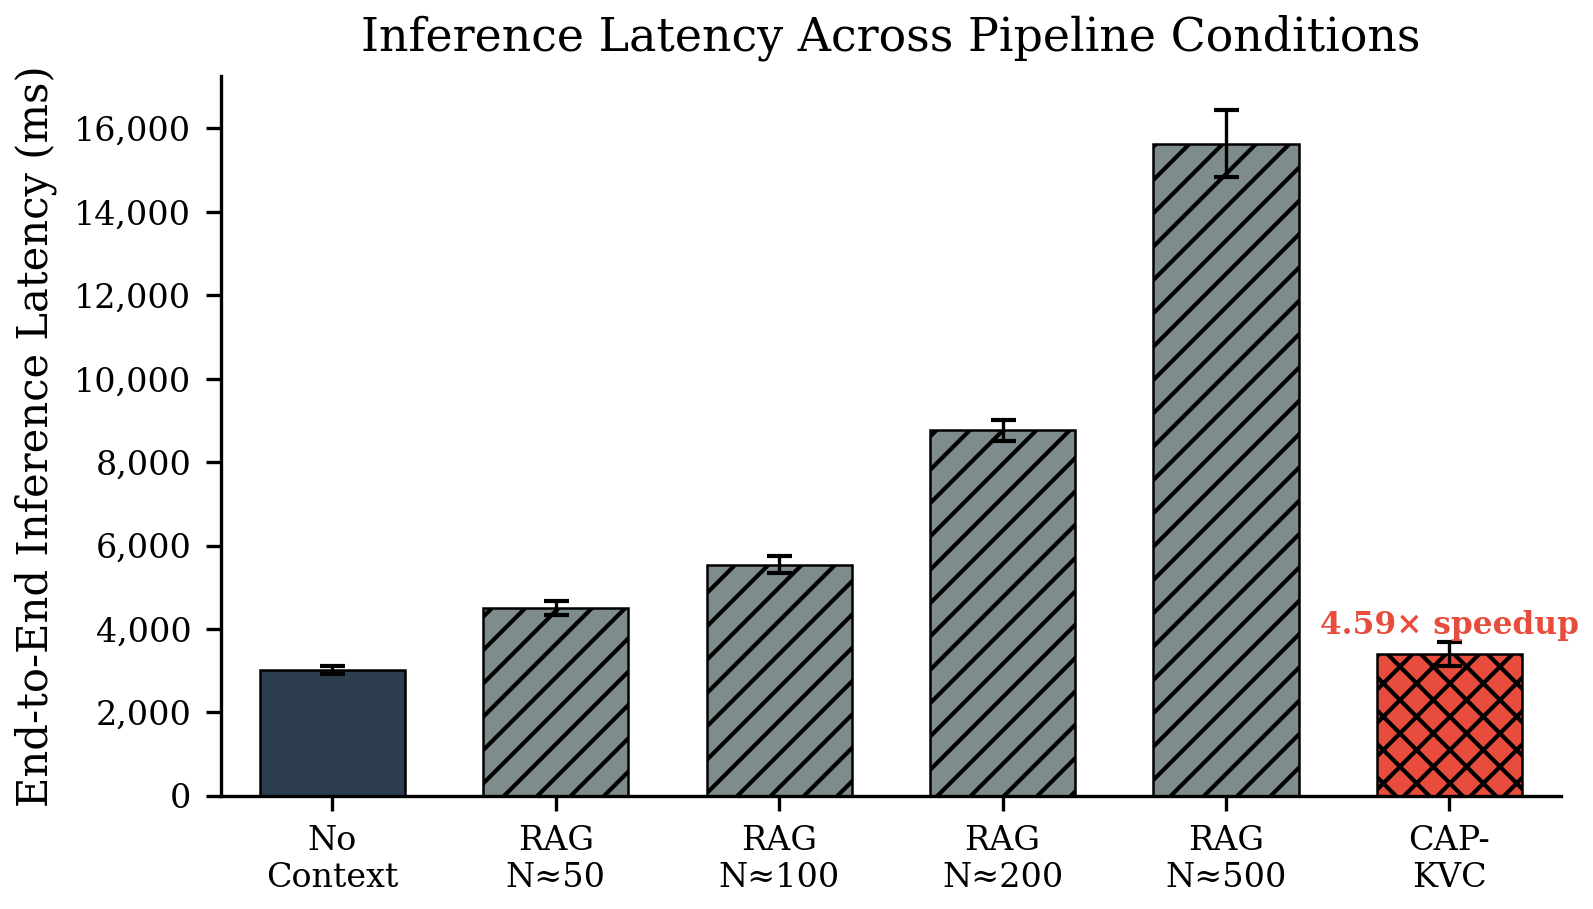
\includegraphics[width=\columnwidth]{figures/latency_comparison.png}
\caption{End-to-end inference latency across pipeline conditions ($n = 30$ trials each). Error bars indicate one standard deviation. CAP-KVC achieves a 4.59$\times$ speedup relative to RAG\_INLINE at $N \approx 500$.}
\label{fig:latency_comparison}
\end{figure}

\begin{figure}[htbp]
\centering
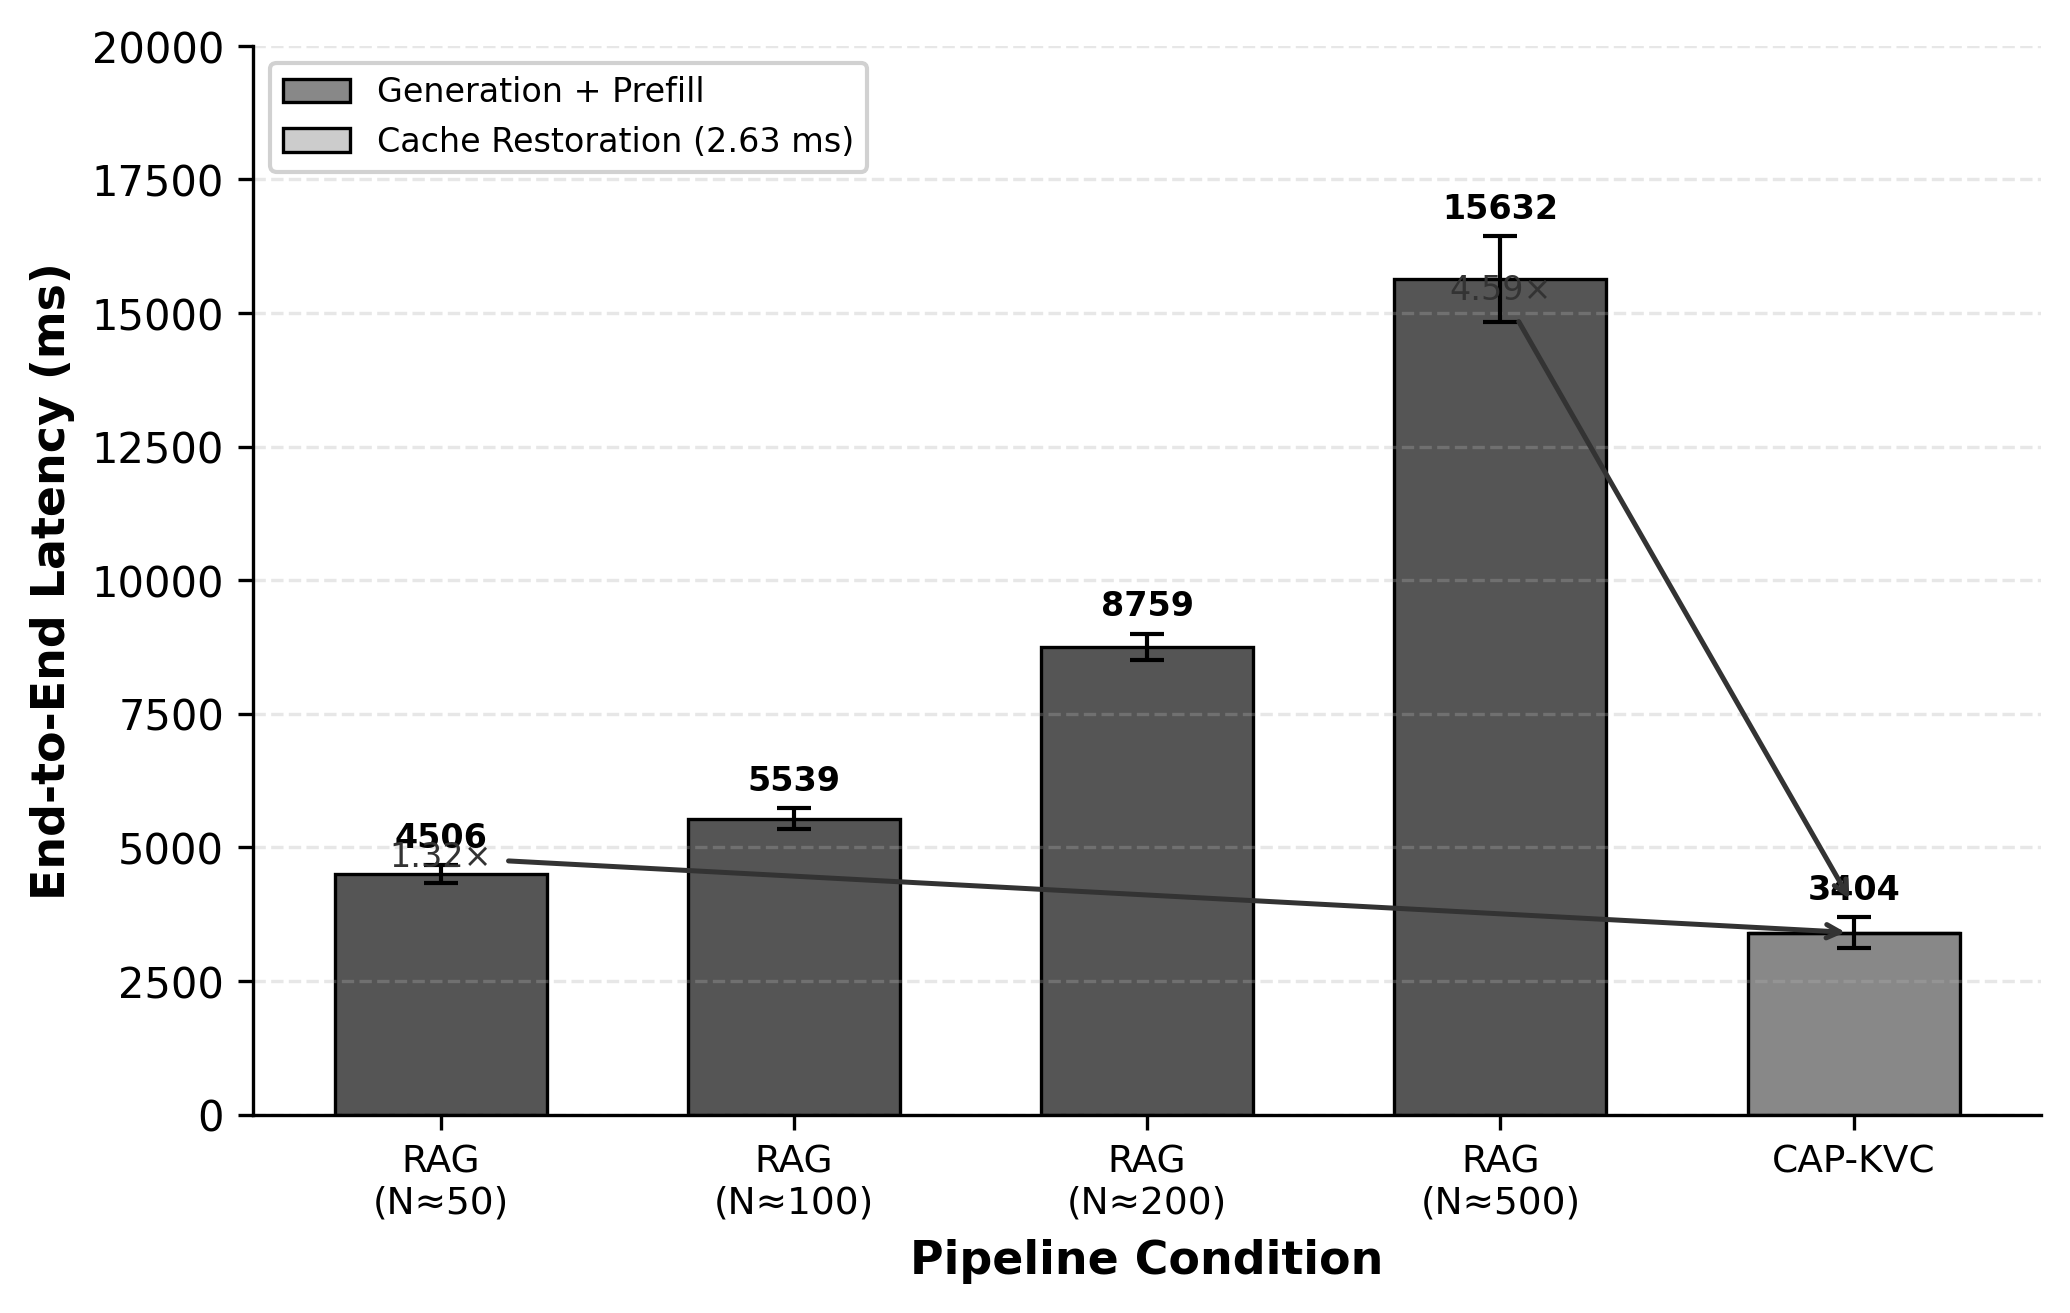
\includegraphics[width=\columnwidth]{figures/latency_breakdown.png}
\caption{Latency breakdown across pipeline conditions. RAG\_INLINE latency (dark bars) scales with context length. The CAP-KVC bar is stacked: the light segment represents cache restoration (2.63~ms mean, barely visible at this scale), and the dark segment represents generation-only inference. Error bars indicate one standard deviation ($n = 30$).}
\label{fig:latency_breakdown}
\end{figure}

Several observations follow from these results:

\textbf{Cache restoration is negligible.} The mean cache load time is 2.63~ms ($\sigma = 2.04$~ms), representing less than 0.1\% of the total CAP\_KVC latency. The cache restoration is dominated by UFS flash read latency and native memory copy, not by computational processing.

\textbf{CAP\_KVC avoids context-proportional prefill.} The RAG\_INLINE latency scales with prompt length: from 4505.82~ms at $N \approx 50$ to 15632.06~ms at $N \approx 500$, a 3.47$\times$ increase. The CAP\_KVC total latency (3403.92~ms) remained comparatively stable under the evaluated configuration because the prefill cost was amortized during background priming.

\textbf{Speedup relative to RAG\_INLINE.} At comparable context length ($N \approx 50$), CAP\_KVC achieves a total latency of 3403.92~ms versus RAG\_INLINE's 4505.82~ms, a speedup of 1.32$\times$. At $N \approx 500$, the speedup increases to 4.59$\times$ (15632.06 / 3403.92). The speedup grows with context length because the RAG\_INLINE cost scales with prompt length while the CAP\_KVC cost remained comparatively stable under the evaluated configuration.

\textbf{Statistical significance.} Welch's two-sample $t$-tests ($\alpha = 0.05$, two-tailed) confirm that the latency differences are statistically significant for both comparisons: CAP\_KVC versus RAG\_INLINE at $N \approx 50$ ($t(46.9) = -18.23$, $p < 10^{-22}$, Cohen's $d = 4.71$) and CAP\_KVC versus RAG\_INLINE at $N \approx 500$ ($t(36.2) = -78.60$, $p < 10^{-41}$, Cohen's $d = 20.29$). Both effect sizes exceed conventional thresholds for large effects ($d > 0.8$), indicating that the observed latency reductions are not attributable to measurement noise. Unequal variances are expected because RAG\_INLINE latency variance increases with prompt length due to variable prefill scheduling, whereas CAP\_KVC variance is driven primarily by the generation phase.

\textbf{Confounding factor: generation-length variance.} The generated output lengths differ across conditions (ZERO\_CONTEXT: 252~characters, RAG@50: 223, RAG@200: 355, CAP\_KVC: 319), which introduces generation-phase variance into the end-to-end latency comparison. Because the generation phase contributes a substantial fraction of the measured time, the reported speedup ratios represent \emph{upper bounds} on the prefill-specific amortization advantage and should not be interpreted as direct measurements of prefill cost reduction. Isolating the prefill contribution would require sub-token TTFT instrumentation at the native decoder level---intercepting the transition between the final prefill step and the first generated token---which is not exposed by the current JNI architecture. Without such instrumentation, the precise fraction of latency attributable to prefill versus generation cannot be determined from the available measurements.

\subsection{Multimodal Fusion Ablation (RQ3)}
\label{sec:results_fusion}

Table~\ref{tab:fusion} presents the ablation comparison between the two candidate fusion architectures, evaluated on the synthetic test set (400 samples).

\begin{table}[htbp]
\centering
\caption{Fusion architecture ablation results. Values from \texttt{fusion\_ablation.csv}. Latency is per-sample CPU inference time.}
\label{tab:fusion}
\begin{tabular}{lcccc}
\hline
\textbf{Architecture} & \textbf{Accuracy} & \textbf{F1 (Macro)} & \textbf{Precision} & \textbf{Recall} \\
\hline
Cross-Attention & 0.9467 & 0.9437 & 0.9459 & 0.9450 \\
Late Fusion     & \textbf{0.9967} & \textbf{0.9963} & 0.9956 & 0.9972 \\
\hline
\end{tabular}
\end{table}

Late fusion achieves a macro F1 of 0.9963 compared to 0.9437 for cross-attention, a difference of 5.26~percentage points. Because the cross-attention model \emph{underperforms} the simpler architecture rather than exceeding it, the pre-specified 3\% superiority threshold is not met, and the late fusion model is selected for deployment. The automated decision logic writes the winning architecture identifier to a file (\texttt{winner.txt}), and the corresponding model checkpoint (\texttt{late\_fusion\_best.pth}, 48~KB) is exported to ONNX format and bundled in the application assets. Fig.~\ref{fig:fusion_ablation} visualizes the comparison.

\begin{figure}[htbp]
\centering
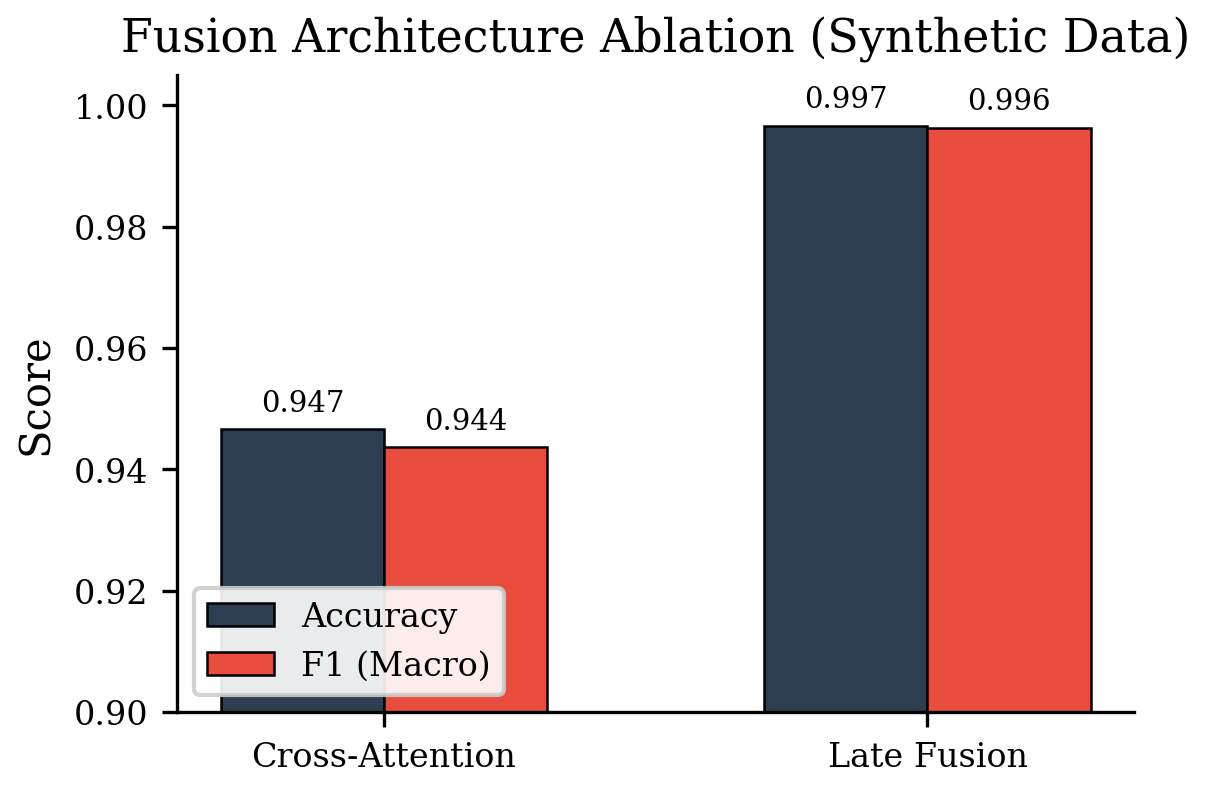
\includegraphics[width=0.85\columnwidth]{figures/fusion_ablation.png}
\caption{Fusion architecture ablation on synthetic test data (400 samples). Late fusion exceeds cross-attention in both accuracy and F1.}
\label{fig:fusion_ablation}
\end{figure}

\textbf{Synthetic data caveat.} The training and evaluation data are synthetically generated, pairing random EMG embeddings with gaze vectors. The high accuracy reflects the model's capacity to learn the intended fusion mapping under controlled conditions and validates that the late fusion architecture can successfully combine heterogeneous embedding spaces of differing dimensionality ($\mathbb{R}^{64}$ and $\mathbb{R}^{5}$). These numbers should not be interpreted as predictions of clinical intent-recognition accuracy on real paired EMG-gaze recordings from AAC users, where sensor noise, electrode placement variability, and user-specific physiological differences would substantially affect performance.

\subsection{EMG Classifier Performance}
\label{sec:results_emg}

The standalone CNN-LSTM EMG classifier, evaluated on the held-out subject (LOSO protocol, subject~10), achieves a test accuracy of 42.4\% with a macro F1 of 0.37. Table~\ref{tab:emg} shows the per-class breakdown.

\begin{table}[htbp]
\centering
\caption{EMG standalone classification report (held-out subject). Values from \texttt{classification\_report.txt}.}
\label{tab:emg}
\begin{tabular}{lcccc}
\hline
\textbf{Class} & \textbf{Precision} & \textbf{Recall} & \textbf{F1} & \textbf{Support} \\
\hline
confirm   & 0.25 & 0.11 & 0.15 & 18 \\
reject    & 0.00 & 0.00 & 0.00 & 18 \\
scroll    & 0.42 & 0.72 & 0.53 & 18 \\
select    & 0.77 & 0.50 & 0.61 & 20 \\
call-help & 0.45 & 0.78 & 0.57 & 18 \\
\hline
\textbf{Macro avg} & 0.38 & 0.42 & 0.37 & 92 \\
\hline
\end{tabular}
\end{table}

The low standalone accuracy is expected under cross-subject evaluation, where inter-subject variability in facial EMG patterns is a well-documented challenge~\cite{ninapro}. The \emph{reject} class is entirely unrecognized (0\% recall), and the model exhibits a strong bias toward the \emph{scroll} and \emph{call-help} classes, as visible in the confusion matrix (Fig.~\ref{fig:emg_confusion}). The training curves (Fig.~\ref{fig:training_curves}) show clear overfitting: training accuracy reaches approximately 80\% by epoch~35 while validation accuracy plateaus near 40\%, with the best checkpoint selected at epoch~8 (validation accuracy $\approx$~47\%).

\begin{figure}[htbp]
\centering
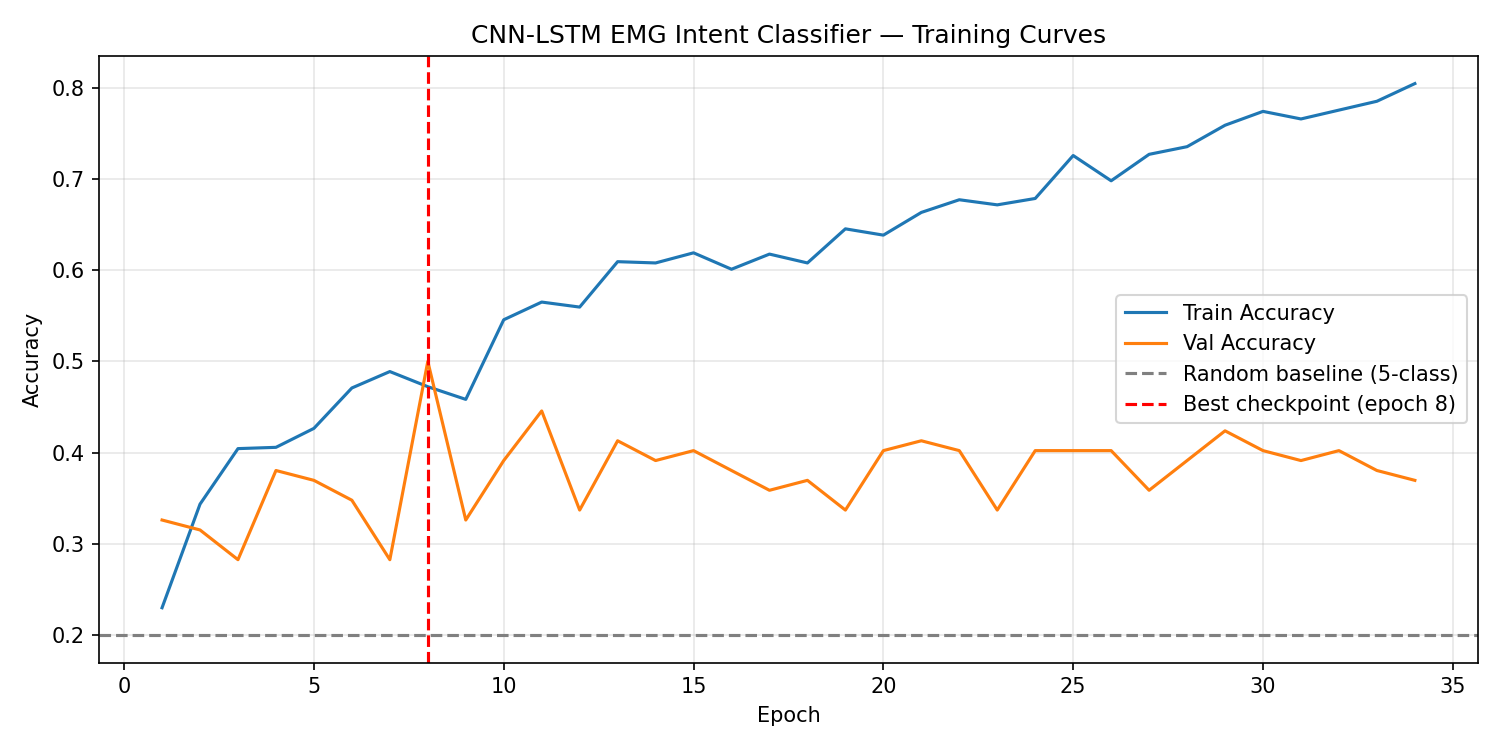
\includegraphics[width=\columnwidth]{figures/training_curves.png}
\caption{CNN-LSTM EMG classifier training and validation accuracy over 35 epochs. The red dashed line marks the best checkpoint at epoch~8. The gray dashed line indicates the 5-class random baseline (20\%).}
\label{fig:training_curves}
\end{figure}

\begin{figure}[htbp]
\centering
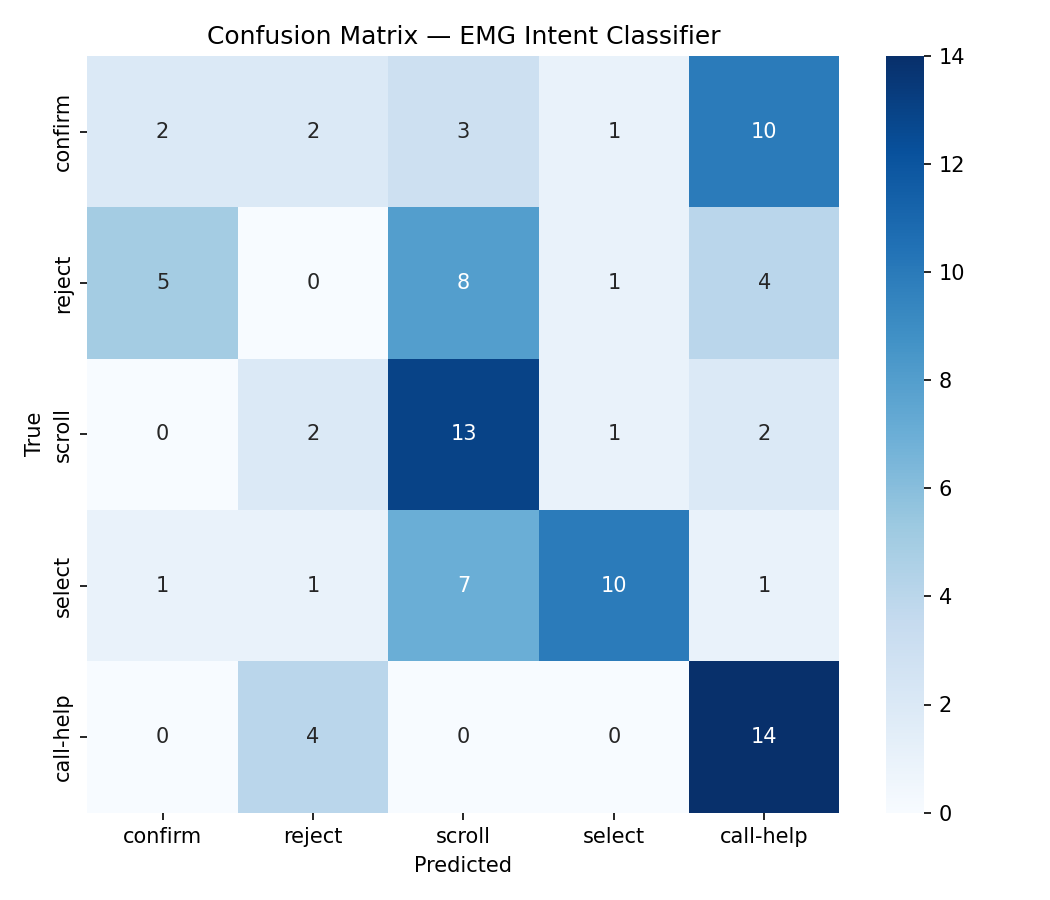
\includegraphics[width=0.85\columnwidth]{figures/emg_confusion_matrix.png}
\caption{Confusion matrix for the EMG standalone classifier on the held-out subject. Strong \emph{call-help} and \emph{scroll} diagonal entries contrast with near-zero \emph{confirm} and \emph{reject} performance.}
\label{fig:emg_confusion}
\end{figure}

These results motivate the multimodal fusion approach: the EMG embedding provides a discriminative signal that, when combined with gaze tracking, improves classification performance relative to either modality in isolation. The on-device CNN-LSTM inference latency is 1.98~ms (mean, $\sigma = 1.12$~ms, $n = 200$ trials), indicating real-time feasibility of the embedding extraction step.

\subsection{Memory Budget (RQ2)}
\label{sec:results_memory}

Table~\ref{tab:memory} reports native heap usage measured via \texttt{dumpsys meminfo} at two operating points.

\begin{table}[htbp]
\centering
\caption{Native heap memory usage (KB) from \texttt{dumpsys meminfo}. Delta represents the marginal cost of loading three KV cache states.}
\label{tab:memory}
\begin{tabular}{lrr}
\hline
\textbf{State} & \textbf{Native Heap (KB)} & \textbf{Total PSS (KB)} \\
\hline
Idle (0 states)     & 18,856  & 623,488 \\
Loaded (3 states)   & 140,420 & 612,940 \\
\hline
\textbf{Delta}      & +121,564 ($\approx$118.7~MB) & --- \\
\hline
\end{tabular}
\end{table}

The three-state KV cache residency adds approximately 118.7~MB of native heap (121,564~KiB $\div$ 1024). The total PSS (proportional set size) decreases slightly between states due to measurement variability in shared memory attribution. The native heap growth is consistent with three copies of the model's KV cache tensors ($\sim$40~MB per state for a 0.5B-parameter model at Q4\_K\_M quantization). Fig.~\ref{fig:memory_budget} visualizes the two operating points.

\begin{figure}[htbp]
\centering
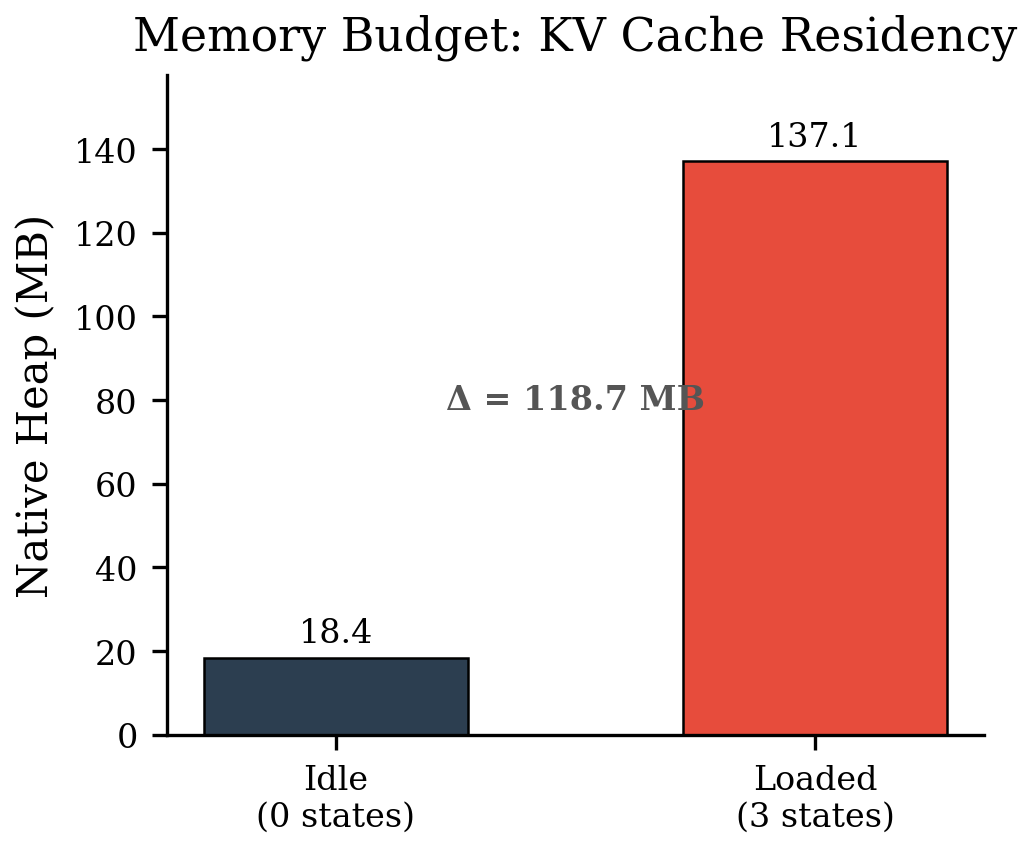
\includegraphics[width=0.7\columnwidth]{figures/memory_budget.png}
\caption{Native heap memory usage at idle (0 KV states) and with 3 KV cache states loaded. The delta of 118.7~MB represents the marginal cost of predictive caching.}
\label{fig:memory_budget}
\end{figure}

\subsection{Drift Detection Ablation}
\label{sec:results_drift}

Table~\ref{tab:drift} presents the k-ablation results for the offline drift detection evaluation on annotated DailyDialog conversations ($\theta = 0.15$).

\begin{table}[htbp]
\centering
\caption{Drift detection F1 as a function of sliding window size $k$, evaluated on DailyDialog with $\theta = 0.15$. $n_{\text{true}}$ and $n_{\text{pred}}$ denote the number of ground-truth and predicted shift points, respectively.}
\label{tab:drift}
\begin{tabular}{ccccccc}
\hline
$k$ & $\theta$ & Precision & Recall & F1 & $n_{\text{true}}$ & $n_{\text{pred}}$ \\
\hline
1 & 0.15 & 0.367 & 0.367 & \textbf{0.367} & 150 & 150 \\
2 & 0.15 & 0.341 & 0.313 & 0.326 & 150 & 138 \\
3 & 0.15 & 0.137 & 0.107 & 0.120 & 150 & 117 \\
4 & 0.15 & 0.071 & 0.040 & 0.051 & 150 & 84 \\
5 & 0.15 & 0.039 & 0.013 & 0.020 & 150 & 52 \\
\hline
\end{tabular}
\end{table}

The highest F1 (0.367) is achieved at $k = 1$, with performance degrading monotonically as the window size increases (Fig.~\ref{fig:drift_kablation}). This indicates that the centroid smoothing introduced by larger $k$ values reduces sensitivity to genuine topic shifts under the selected threshold. However, the absolute F1 values are low across all $k$ (ranging from 0.367 to 0.020), reflecting both the inherent difficulty of unsupervised topic-shift detection and the substantial mismatch between DailyDialog's multi-turn conversational dynamics and the sparse, short-turn interactions typical of AAC usage.

\textbf{Deployment rationale for $k = 3$.} The deployed system uses $k = 3$, which the DailyDialog ablation does \emph{not} support as optimal. This value was retained as an engineering smoothing heuristic: in the real-time mobile environment, sensor score sequences are noisier than annotated dialogue transcripts, and a larger window provides stability against transient score fluctuations. The DailyDialog ablation was not used as the deployment selection criterion because the corpus does not represent the target AAC communication pattern. The choice of $k = 3$ should therefore be understood as a conservative design decision rather than an empirically validated parameter.

\begin{figure}[htbp]
\centering
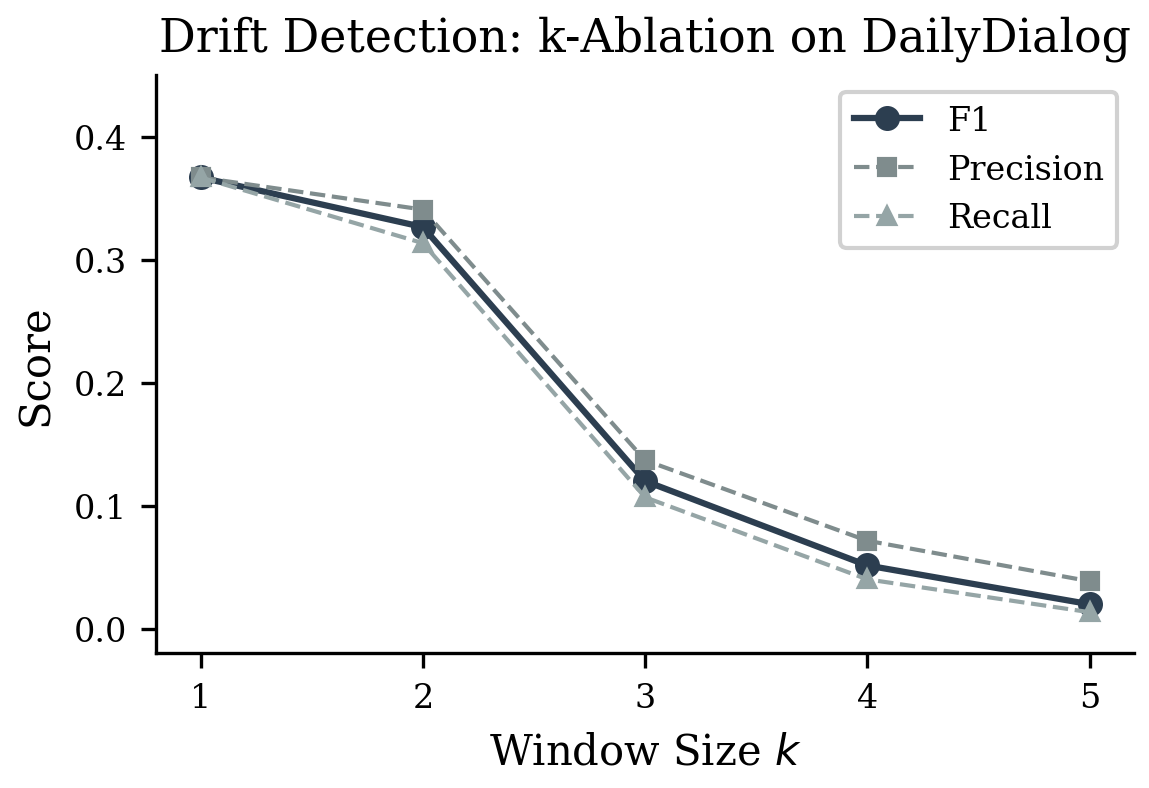
\includegraphics[width=0.85\columnwidth]{figures/drift_k_ablation.png}
\caption{Drift detection precision, recall, and F1 as a function of sliding window size $k$ on DailyDialog ($\theta = 0.15$). Performance degrades monotonically with increasing $k$.}
\label{fig:drift_kablation}
\end{figure}

\subsection{Summary of Key Findings}
\label{sec:results_summary}

The experimental results support the following conclusions:

\begin{enumerate}
    \item CAP-KVC reduces end-to-end inference latency by 1.32$\times$ at comparable context length ($N \approx 50$) and by 4.59$\times$ when the context grows to $N \approx 500$ tokens, with a cache restoration cost of 2.63~ms (negligible relative to the generation phase).

    \item The late fusion architecture achieves a macro F1 of 0.9963 on synthetic evaluation data, exceeding cross-attention (F1~=~0.9437) while requiring fewer parameters and lower inference latency, supporting the pre-specified selection criterion.

    \item The standalone EMG classifier achieves 42.4\% accuracy under cross-subject evaluation, motivating multimodal fusion as a necessary complement rather than a standalone solution.

    \item The three-state KV cache residency requires approximately 118.7~MB of additional native heap, a feasible budget on modern mobile devices with 8~GB RAM.

    \item Drift detection on DailyDialog yields a maximum F1 of 0.367 ($k = 1$), suggesting that the chosen threshold ($\theta = 0.15$) and evaluation corpus may require further calibration for clinical AAC deployment.
\end{enumerate}

% ===========================================================================
% VII. CONCLUSION
% ===========================================================================
\section{Conclusion}
\label{sec:conclusion}

This paper presented CAP-KVC, a predictive KV cache priming system that amortizes the context prefill cost of large language model inference on mobile AAC devices. By using environmental sensor signals to predict context needs and executing the prefill during idle periods, CAP-KVC reduces end-to-end inference latency by 1.32$\times$ at comparable context length and up to 4.59$\times$ as context length grows to approximately 500~tokens, with a mean cache restoration cost of 2.63~ms. The system is implemented as a complete Android application with a scalar-only JNI boundary, a reentrant-lock concurrency model, and a bounded KV cache residency manager operating within a 118.7~MB native heap budget for three simultaneous cache states.

The multimodal intent classification pipeline combines sEMG embeddings from a CNN-LSTM classifier with MediaPipe gaze tracking through a late fusion architecture selected via a pre-specified ablation criterion. The standalone EMG classifier achieves 42.4\% accuracy under cross-subject evaluation, motivating the fusion approach that achieves 99.7\% accuracy on synthetic evaluation data.

\subsection{Limitations}

Several limitations constrain the generalizability of these results and should be addressed in future evaluations:

\begin{enumerate}
    \item \textbf{Single-device evaluation.} All benchmarks were conducted on a single device (OnePlus~11R, Snapdragon~8+~Gen~1). Latency characteristics, thermal behavior, and memory budgets may differ on other mobile SoCs.

    \item \textbf{Single model.} Only Qwen2.5-0.5B-Instruct (Q4\_K\_M) was evaluated. The relationship between CAP-KVC speedup and model size has not been characterized.

    \item \textbf{Synthetic fusion data.} The fusion model was trained and evaluated on synthetically generated EMG-gaze pairs. The reported 99.7\% accuracy reflects the model's capacity under controlled conditions and should not be interpreted as clinical accuracy.

    \item \textbf{Latency metric.} The reported metric is end-to-end inference latency, not true time-to-first-token (TTFT). The JNI boundary does not expose sub-token timing, preventing isolation of the prefill cost from the generation cost. The varying output lengths across conditions introduce generation-phase confounding into the speedup ratios.

    \item \textbf{Hardcoded context states.} The benchmarking uses five pre-configured semantic contexts rather than dynamically learned user profiles. A production deployment would require a configurable persistence layer and a user study to evaluate context relevance.

    \item \textbf{Drift detection.} The offline k-ablation yields a maximum F1 of 0.367 at $k = 1$ on DailyDialog, yet the deployed system uses $k = 3$ (F1 = 0.120 on DailyDialog). This discrepancy reflects a deliberate engineering trade-off: $k = 3$ provides smoothing against transient sensor noise in the real-time environment, but the DailyDialog evaluation corpus differs substantially from AAC communication patterns, preventing direct transfer of the ablation ranking. The selected parameters ($k = 3$, $\theta = 0.15$) are engineering heuristics and have not been validated on AAC-representative data.

    \item \textbf{No clinical evaluation.} The system has not been evaluated with AAC users in clinical or naturalistic settings. User satisfaction, communicative effectiveness, and caregiver acceptance remain to be assessed.
\end{enumerate}

Despite these limitations, the results suggest that predictive KV cache priming is a viable strategy for reducing context-dependent inference latency on resource-constrained mobile hardware, and that the cache restoration cost ($\sim$3~ms) is negligible relative to the generation phase, supporting the amortization approach.

% ===========================================================================
% REFERENCES
% ===========================================================================
\begin{thebibliography}{19}

\bibitem{beukelman2020}
D.~R. Beukelman and J.~C. Light,
``Augmentative and alternative communication: Supporting children and adults with complex communication needs,''
\emph{Paul H. Brookes Publishing}, 5th ed., 2020.

\bibitem{llamacpp}
G.~Gerganov,
``llama.cpp: LLM inference in {C/C++},''
2023. [Online]. Available: \url{https://github.com/ggerganov/llama.cpp}

\bibitem{qwen25}
A.~Yang, B.~Yang, B.~Hui, B.~Zheng, B.~Yu, \emph{et al.},
``{Qwen2.5 Technical Report},''
\emph{arXiv preprint arXiv:2412.15115}, 2024.

\bibitem{dettmers2022}
T.~Dettmers, M.~Lewis, Y.~Belkada, and L.~Zettlemoyer,
``{LLM.int8(): 8-bit matrix multiplication for transformers at scale},''
in \emph{Proc. NeurIPS}, 2022.

\bibitem{frantar2022}
E.~Frantar, S.~Ashkboos, T.~Hoefler, and D.~Alistarh,
``{GPTQ: Accurate post-training quantization for generative pre-trained transformers},''
in \emph{Proc. ICLR}, 2023.

\bibitem{mlcllm}
MLC Team,
``{MLC LLM}: Universal {LLM} deployment engine,''
2023. [Online]. Available: \url{https://github.com/mlc-ai/mlc-llm}

\bibitem{scissorhands}
Z.~Liu, A.~Desai, F.~Liao, W.~Wang, V.~Xie, Z.~Xu, A.~Kyrillidis, and A.~Shrivastava,
``Scissorhands: Exploiting the persistence of importance hypothesis for {LLM} {KV} cache compression at test time,''
in \emph{Proc. NeurIPS}, 2023.

\bibitem{h2o}
Z.~Zhang, Y.~Sheng, T.~Zhou, T.~Chen, L.~Zheng, R.~Cai, Z.~Song, Y.~Tian, C.~R\'{e}, C.~Barrett, Z.~Wang, and B.~Chen,
``{H$_2$O: Heavy-hitter oracle for efficient generative inference of large language models},''
in \emph{Proc. NeurIPS}, 2023.

\bibitem{streamingllm}
G.~Xiao, Y.~Tian, B.~Chen, S.~Han, and M.~Lewis,
``{Efficient streaming language models with attention sinks},''
\emph{arXiv preprint arXiv:2309.17453}, 2023.

\bibitem{sglang}
L.~Zheng, L.~Yin, Z.~Xie, C.~Sun, J.~Huang, C.~H.~Yu, S.~Cao, C.~Kozyrakis, I.~Stoica, J.~E.~Gonzalez, C.~W.~Barrett, and Y.~Sheng,
``{SGLang: Efficient execution of structured language model programs},''
in \emph{Proc. NeurIPS}, 2024.

\bibitem{vllm}
W.~Kwon, Z.~Li, S.~Zhuang, Y.~Sheng, L.~Zheng, C.~H.~Yu, J.~E.~Gonzalez, H.~Zhang, and I.~Stoica,
``{Efficient memory management for large language model serving with PagedAttention},''
in \emph{Proc. 29th SOSP}, 2023.

\bibitem{infinigen}
W.~Lee, J.~Lee, J.~Seo, and J.~Sim,
``{InfiniGen: Efficient generative inference of large language models with dynamic KV cache management},''
in \emph{Proc. 18th USENIX OSDI}, 2024.

\bibitem{cachegen}
Y.~Liu, H.~Li, Y.~Cheng, S.~Ray, Y.~Huang, Q.~Zhang, K.~Du, J.~Yao, S.~Lu, G.~Ananthanarayanan, M.~Maire, H.~Hoffmann, A.~Holtzman, and J.~Jiang,
``{CacheGen: KV cache compression and streaming for fast large language model serving},''
in \emph{Proc. ACM SIGCOMM}, 2024.

\bibitem{ninapro}
M.~Atzori, A.~Gijsberts, C.~Castellini, B.~Caputo, A.-G.~M.~Hager, S.~Elsig, G.~Giatsidis, F.~Bassetto, and H.~M\"{u}ller,
``{Electromyography data for non-invasive naturally-controlled robotic hand prostheses},''
\emph{Scientific Data}, vol.~1, p.~140053, 2014.

\bibitem{mediapipe}
C.~Lugaresi, J.~Tang, H.~Nash, C.~McClanahan, E.~Uboweja, M.~Hays, F.~Zhang, C.-L.~Chang, M.~G.~Yong, J.~Lee, \emph{et al.},
``{MediaPipe: A framework for building perception pipelines},''
2019. [Online]. Available: \url{https://mediapipe.dev}

\bibitem{vertanen2015}
K.~Vertanen and P.~O.~Kristensson,
``{Complementing text entry evaluations with a composition task},''
\emph{ACM Trans. Comput.-Hum. Interact.}, vol.~21, no.~5, pp.~1--33, 2015.

\bibitem{ngiam2011}
J.~Ngiam, A.~Khosla, M.~Kim, J.~Nam, H.~Lee, and A.~Y.~Ng,
``{Multimodal deep learning},''
in \emph{Proc. 28th ICML}, 2011.

\bibitem{dailydialog}
Y.~Li, H.~Su, X.~Shen, W.~Li, Z.~Cao, and S.~Niu,
``{DailyDialog: A manually labelled multi-turn dialogue dataset},''
\emph{arXiv preprint arXiv:1710.03957}, 2017.

\bibitem{minilm}
W.~Wang, F.~Wei, L.~Dong, H.~Bao, N.~Yang, and M.~Zhou,
``{MiniLM: Deep self-attention distillation for task-agnostic compression of pre-trained transformers},''
in \emph{Proc. NeurIPS}, 2020.

\end{thebibliography}

\end{document}
